%! TeX program = lualatex
%%%%%%%%%%%%%%%%%%%%%%%%%%%%%%%%%%%%%%%%%
% Simple Article
% Integrated article template with simple for make4ht
% LaTeX Class
% Version 1.0 (10/11/20)
%
% This class originates by:
% Vel and  Nicolas Diaz
%
% Authors:
% Muhammad Uliah Shafar
%
%
% Free License:
%
%
%%%%%%%%%%%%%%%%%%%%%%%%%%%%%%%%%%%%%%%%%
\documentclass[11pt]{simartadv} % Font size (can be 10pt, 11pt or 12pt)

%----------------------------------------------------------------------------------------
%	TITLE SECTION
%----------------------------------------------------------------------------------------
% MAIN TITLE SECTION
\title{
\textbf{Lorem Ipsum Lorem Ipsum \\
Lorem Ipsum Lorem Ipsum Lorem Ipsum} \\
\textbf{{Lorem Ipsum Lorem Ipsum \\}}
} % Title and subtitle
%\date{\textbf{\DTMtoday}}
\date{\textbf{\today}}
\author{
\begin{tabular}{@{}ll@{}}
	Nama & : Muhammad Uliah Shafar\\
	NIM & : 21020119420029\\
\end{tabular}
}

%----------------------------------------------------------------------------------------
% OTHER TITLE SECTION

%\title{\textbf{Sistem Sarana dan Prasarana Jl. Pinggir Laut} \\ {\Large\itshape Infrastructure of Waterfront Parepare City}} % Title and subtitle

%\author{\textbf{Uliah Shafar} \\ \textit{Universitas Diponegoro}} % Author and institution

%\date{\today} % Date, use \date{} for no date

%----------------------------------------------------------------------------------------



\begin{document}

%----------------------------------------------------------------------------------------
%	ESSAY BODY
%----------------------------------------------------------------------------------------
\section{Abstract}
Tujuan penelitian ini adalah menganalisis preferensi pengunjung terhadap ruang publik di tepi laut. 
Kawasan tepi laut memiliki peran yang sangat penting untuk kesejahteraan masyarakat perkotaan saat ini.
Seiring waktu, terjadi peningkatkan permintaan masyarakat terhadap ruang publik berbasis di tepi laut yang mendorong konsep desain tepi laut yang sesuai dengan kebutuhan masyarkat. 
Pemahaman preferensi terhadap ruang publik yang sukses mampu memberikan wawasan kepada pemangku kepentingan atau perencana dalam mendesain ruang publik yang memenuhi kebutuhan masyarakat.
Penelitian ini akan melengkapi kekurangan studi preferensi yang ada di tepi laut.
Objek penelitian ini berada di tepi laut pantai senggol atau saat ini dikenal dengan pantai Parepare, Parepare, Sulawesi Selatan. 
Tepi laut ini memiliki dua ruang yang berbeda dalam satu kawasan. Kedua ruang tersebut masing-masing dinamai dengan ruang A dan Ruang B. Perbedaan tersebut merupakan alasan untuk mengetahui preferensi pengunjung. Pengetahuan ini akan menjelaskan kebutuhan pengunjung sebagai konsep dalam merancang yang efektif sebuah ruang publik. 
Metode penelitian ini adalah campuran. Sementara, desain penelitian ini adalah \textit{cross-sectional} dengan menggunakan crosstabulasi dan analisis gambar biplot. 
Melalui survei kuesioner, responden yang terdiri dari 85 orang ini diminta untuk memilih satu diantara dua ruang yang sangat disukai, beserta alasan menyukai ruang tersebut berdasarkan aspek dan elemen-elemen ruang. 
Hasilnya menunjukkan 66\% responden menyukai ruang A dan 34\% menyukai ruang B. Alasan kebanyakan responden adalah berkaitan dengan aspek fasilitas. Selain itu, banyak dari mereka menyukai jalan yang lebar dibanding elemen-elemen ruang lainnya. Oleh karena itu, desain dan elemen yang tersedia pada ruang B tidak memenuhi preferensi dan kebutuhan kebanyakan pengunjung dan juga tidak berkontribusi terhadap kesejahteraan masyarakat.


The purpose of this research paper is to analyze the preference of visitors on waterfront public space.
The waterfront area has an important role for the current city society well-being.
As time goes by, there is an increasing demand of people on waterfront based public space that encourages waterfront design concept and fits with the people needs.
Understanding the preference on public space successfully will hand an insight to stakeholders and planners on designing public space that fulfill people needs.
This research will complete the scarcity of the available preference study in waterfront.
This research object are located in Senggol beach waterfront or currently known as Parepare beach, Parepare, South Sulawesi.
This waterfront has two difference spaces in an area. Both spaces are named as A space and B space. This distinction is the reason why acknowledging the visitor preference. This acknowledgment will explain the needs of the visitor as a concept of public space effective planning.  
This research method is mixed-method. Furthermore, this research design is cross-sectional using cross tabulation and biplot image analysis.
Through questionnaire survey, respondents which consist of 85 people were asked to choose one of the spaces which they liked, including their reason to like it according to aspects and elements of the space.
The result shows that 66\% respondents like A space and 35\% like B space. The reason of many respondents is regarding facilities aspect. Also, many respondents like a wide path more than other space elements. Therefore, available designs and elements in B space are not satisfied most respondent's preference and need and also do not contribute to people's well-being.

Sehingga meningkatkan permintaan masyarakat terhadap ruang publik di tepi laut. 

Munculnya permintaan masyarakat terhadap ruang publik yang berbasis di tepi laut mendorong konsep desain tepi laut yang sesuai dengna kebutuhan masyarakat.


\section{Pendahuluan}

Tepi laut merupakan sebuah ruang perkotaan yang sangat memerlukan pengembangan secara terus menerus \citep{shamsuddin2013}. Ruang ini mempunyai sejumlah karakteristik-karakteristik yang unik oleh karena air merupakan sumber kehidupan \citep{yassin2010}. Pengembangan tepi laut yang sukses mempertimbangkan sejumlah aspek yaitu keberagaman, interaksi komunitas, kenyamanan dan keamanan, lingkungan dan keberlanjutan \citep{hussein2014}. Pengembangan yang sukses oleh tepi laut akan mengantarkan masyarakat menuju ke kawasan tepi laut dari pusat kota \citep{hoyle2001}.

Pembahasan terkait pengembangan tepi laut belakangan ini menjadi topik yang hangat di Indonesia. Terdapat sejumlah pengembangan yang terjadi di sejumlah daerah seperti proyek reklamasi di Makassar dan Manado \citep{andi2017,fhuh2017,tungka2012}, desain lanskap tepi laut di sungai Cikapundung \citep{ainy2016}, dan pengembangan ulang tepi laut pada tahun 1995 sepanjang 32 km di Jakarta \citep{pramesti2017}. 
Pengembagan tepi laut juga terjadi di kota Parepare, salah satunya berada di tepi laut Senggol \citep{tri2020}.

Tepi laut senggol merupakan daya tarik wisata masyarakat kota Parepare sejak lama. Orang-orang dapat menikmati pemandangan yang indah dan ditemani dengan makanan-makanan khas pedagang kaki lima. Selain itu, mereka juga dapat berenang di laut. Aktivitas-aktivitas tersebut yaitu interaksi dengan air menjadi bagian terpenting dalam pengembangan tepi laut \citep{davidowich1998}. \cite{eldeeb2015} menambahkan penggunaan beragam akan berkontribusi terhadap kesuksesssan sebuah tepi laut.

Pada dasarnya, tepi laut merupakan sebuah ruang yang dapat meningkatkan kualitas hidup seseorang dengan cara memenuhi kebutuhan masyarakat \citep{kim2012}.
Untuk memenuhi kebutuhan tersebut secara efektif, maka pemangku kebijakan dan perencana kota dalam mendesain ruang publik memerlukan pemahaman preferensi terhadap ruang publik yang lebih baik \citep{madureira2018}.
Preferensi terhadap ruang adalah ungkapan keinginan seseorang terhadap suatu ruang \citep{zhang2006}. Ungkapan keinginan ini melekat atau ditimbulkan oleh sebuah elemen ruang perkotaan \citep{knox2014}. Menurut \cite{alves2008}, elemen ruang merupakan bagian fisik dari sebuah ruang publik yang termasuk dalam tatanan ruang publik itu sendiri.

Penelitian terkait preferensi pengunjung terhadap ruang publik di sekitar kawasan tepi laut masih kurang. Hanya ada beberapa penelitian yang membahas preferensi terhadap taman kota \citep{alves2008,devysandra2012,dwiputra2017,madureira2018}, taman publik untuk umum  \citep{grilli2020}, dan ruang publik kampus \citep{zhang2006}. Sehingga penelitian ini diharapkan mampu melengkapi kekurangan studi preferensi tersebut.

Beberapa tahun yang lalu, pengembangan tepi laut Senggol ini selesai. Pengembangan ini menghasilkan dua jenis ruang yang berbeda. Untuk memudahkan penelitian, peneliti menyebut ruang yang satu sebagai ruang A, sedangkan ruang lainnya sebagai ruang B. Kedua ruang ini memiliki sejumlah perbedaan baik dari segi elemen-elemen ruang, aktivitas, dan lain-lain.

Ruang A lebih dikenal dengan tatanan dan elemen buatan yang mewah dan lengkap. Sedangkan ruang B lebih dikenal dengan tatanan dan elemen yang terlihat lebih alami dengan sedikit elemen buatan. Sehingga, kedua ruang ini memunculkan kondisi yang kontras yang membuat orang berpeluang untuk memilih satu ruang daripada lainnya. Kondisi ini dalam kurung waktu tertentu akan menghasilkan ketidakselarasan dimana ruang satu akan terlihat lebih berhasil dalam menarik pengunjung daripada ruang lainnya. Ketidakselaran jumlah pengunjung yang mungkin terjadi ini akan membuat kawasan secara keseluruhan tidak optimal \citep{sari2015}. Menurut \cite{madureira2018}, pemahaman preferensi akan menjawab permasalahan tersebut dengan cara menjelaskan kebutuhan-kebutuhan pengunjung.



\section{Metode Penelitian}
\label{sub:metpen}

Penelitian ini bertujuan untuk menganalisis preferensi pengunjung terhadap ruang di tepi laut Senggol. Tujuan tersebut dapat tercapai dengan menerapkan pendekatan penelitian. Penelitian ini menerapkan pendekatan kualitatif dan kuantitatif \textit{(mixed-method)}. Menurut \cite{creswell2016}, pendekatan kualitatif merupakan gambaran keseluruhan dari sebuah fenomena yang diambil dari pemahaman dan penglihatan secara langsung sebuah fenomena dalam objek penelitian dengan sejumlah sumber yang tersedia. Dalam penelitian ini, fenomena tersebut adalah kecenderungan pengunjung dalam memilih ruang. Sedangkan pendekatan kuantitatif digunakan untuk meneliti populasi atau sampel tertentu berdasarkan variabel penelitian. Lebih lanjut, untuk menilai frekuensi munculnya variabel yang menarik di setiap ruang, maka penelitian ini menerapkan desain analitik dengan pendekatan \textit{cross sectional} sebagai analisis data.

Penelitian ini berlokasi di kawasan tepi laut Senggol di Kota Parepare yang terbentang dari pelabuhan Nusantara hingga Pasar Senggol (lihat gambar \ref{fig:lokzi}). Penelitian ini dilaksanakan setiap hari pada jam 6 - 10 pagi dan 6 - 9 malam karena pada waktu ini menunjukkan keramaian di objek penelitian. Adapun pengumpulan data terbagi atas dua macam data yakni data primer dan sekuder. Pertama, Data primer adalah data yang diambil dari hasil kuesioner yang berdasarkan variabel penelitian. Terakhir, data sekunder merupakan informasi yang telah tersedia oleh pihak atau instansi lain.

\begin{figure}[htpb]
    \centering
    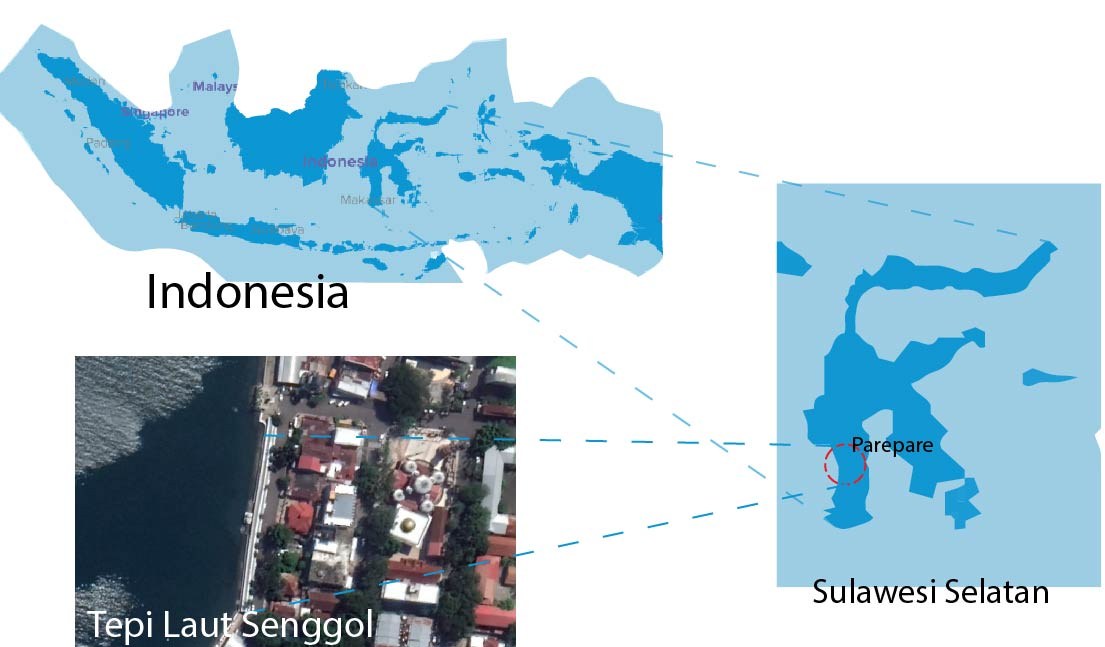
\includegraphics[width=0.86\textwidth]{figures/lokzi}
    \caption{Lokasi Kota Parepare}
    \caption*{Sumber: Dokumentasi, 2022}
    \label{fig:lokzi}
\end{figure}

Penelitian ini menganalisis data dari hasil survei kuesioner terkait preferensi pengunjung yang disertai dengan alasan memilih elemen-elemen yang disukai. Sebelum menganalisis kedua data yang bersifat kualitatif dan kuantitatif, maka peneliti melakukan reduksi data. Setelah itu, peneliti menganalisis data berdasarkan kedua jenis data tersebut.
Untuk data yang berjenis kualitatif seperti kecenderungan dan deskripsi, peneliti mempelajari makna tema-tema yang terdapat dalam teks responden.
Hasil analisis ini menggambarkan data yang dikategorisasikan sesuai dengan kriteria yang didapatkan.
Untuk data yang berjenis kuantitatif, peneliti memahami karakteristik setiap variabel dengan menggunakan pendekatan \textit{cross-sectional}. Hasilnya mengilustrasikan keragaman preferensi terhadap ruang berdasarkan aspek dan elemen ruang serta latar belakang diantara responden atau kelompok.

Kriteria pada penelitian ini terangkum dalam variabel penelitian. Penelitian ini menggunakan variabel tunggal yang hanya memunculkan variabel untuk di deskripsikan faktor atau unsur didalam setiap gejala dalam variabel tersebut. Variabel penelitian secara detil dapat dilihat pada tabel \ref {tab:varpar}.
\newpage

\begin{table}[hp!]
    \small
    \centering
    \caption{Variabel penelitian}
    \label{tab:varpar}
    \begin{tabular}{p{.23\textwidth}p{.33\textwidth}m{.33\textwidth}}
\toprule
\textbf{Variabel} & \textbf{Sub-Variabel} & \textbf{Indikator}  \\
\midrule
\multirow{5}{*}{Aksesibilitas\tikzmark{ak}} & \tikzmark{jp}Jumlah pohon & Sedikit pohon\\
& & Beberapa pohon\\
\cmidrule{2-3}

& \multirow{2}{*}{\tikzmark{bp}Bentuk pohon} & Cukup rindang\\
& & Rindang\\
\cmidrule{2-3}

& \multirow{2}{*}{\tikzmark{lj}Lebar jalan} & 1-3m\\
\multirow{5}{*}{Keamanan\tikzmark{ke}}& & 3m\\
\cmidrule{2-3}


& \multirow{3}{*}{\tikzmark{pj}Permukaan jalan} & Paving\\
& & Aspal \\
& & Tanah \\
\cmidrule{2-3}

& \multirow{2}{*}{\tikzmark{wb}Warna bunga/tanaman} & satu atau dua warna\\
& & tiga atau lebih warna\\
\cmidrule{2-3}

& \multirow{2}{*}{\tikzmark{jk}Jenis kursi} & Kursi bergerak \\
& & Kursi dinding \\
\cmidrule{2-3}

\multirow{5}{*}{Estetika\tikzmark{es}}& \multirow{2}{*}{\tikzmark{tc}Tingkat cahaya} & Sedang\\
& & Tinggi\\
\cmidrule{2-3}

& \multirow{2}{*}{\tikzmark{oe}Orientasi elemen} & Membelakangi laut\\
& & Menghadap laut\\
\cmidrule{2-3}

& \multirow{2}{*}{\tikzmark{tw}Tempat wisata air} & Tempat memancing\\
& & Tempat berenang\\
\cmidrule{2-3}

\multirow{5}{*}{Fasilitas\tikzmark{fa}}& \multirow{2}{*}{\tikzmark{bap}Bangunan penunjang} & Stan \\
& & Kedai\\
\cmidrule{2-3}

& \multirow{2}{*}{\tikzmark{ea}Elemen air} & Laut tenang\\
& & Laut berombang\\
\bottomrule
\end{tabular}
\end{table}


\begin{tikzpicture}[overlay,remember picture,shorten >=.5pt,shorten <=.5pt, transform canvas={yshift=.25\baselineskip}]
    \draw [->] ({pic cs:ak}) -- ({pic cs:lj});
    \draw [->] ({pic cs:ak}) -- ({pic cs:pj});
    \draw [->] ({pic cs:ke}) -- ({pic cs:bp});
    \draw [->] ({pic cs:ke}) -- ({pic cs:pj});
    \draw [->] ({pic cs:es}) -- ({pic cs:jp});
    \draw [->] ({pic cs:es}) -- ({pic cs:wb});
    \draw [->] ({pic cs:es}) -- ({pic cs:ea});
    \draw [->] ({pic cs:fa}) -- ({pic cs:bp});
    \draw [->] ({pic cs:fa}) -- ({pic cs:jk});
    \draw [->] ({pic cs:fa}) -- ({pic cs:lj});
    \draw [->] ({pic cs:fa}) -- ({pic cs:oe});
    \draw [->] ({pic cs:fa}) -- ({pic cs:tw});
    \draw [->] ({pic cs:fa}) -- ({pic cs:bap});
    \draw [->] ({pic cs:sd}) -- ({pic cs:g});
    \draw [->] ({pic cs:sd}) -- ({pic cs:u});
    \draw [->] ({pic cs:sd}) -- ({pic cs:s});
    \draw [->] ({pic cs:sd}) -- ({pic cs:p});
\end{tikzpicture}

\section{Hasil dan Pembahasan}
\label{sub:hsil}
Respon ruang yang disukai di kawasan tepi laut Senggol memiliki 85 total responden. Dari 85 total responden tersebut, 66\% (56) dari responden menyukai ruang A dan 34\% (29) dari responden menyukai ruang B (lihat gambar \ref{fig:pcr}).

\begin{figure}[hp]
    \centering
    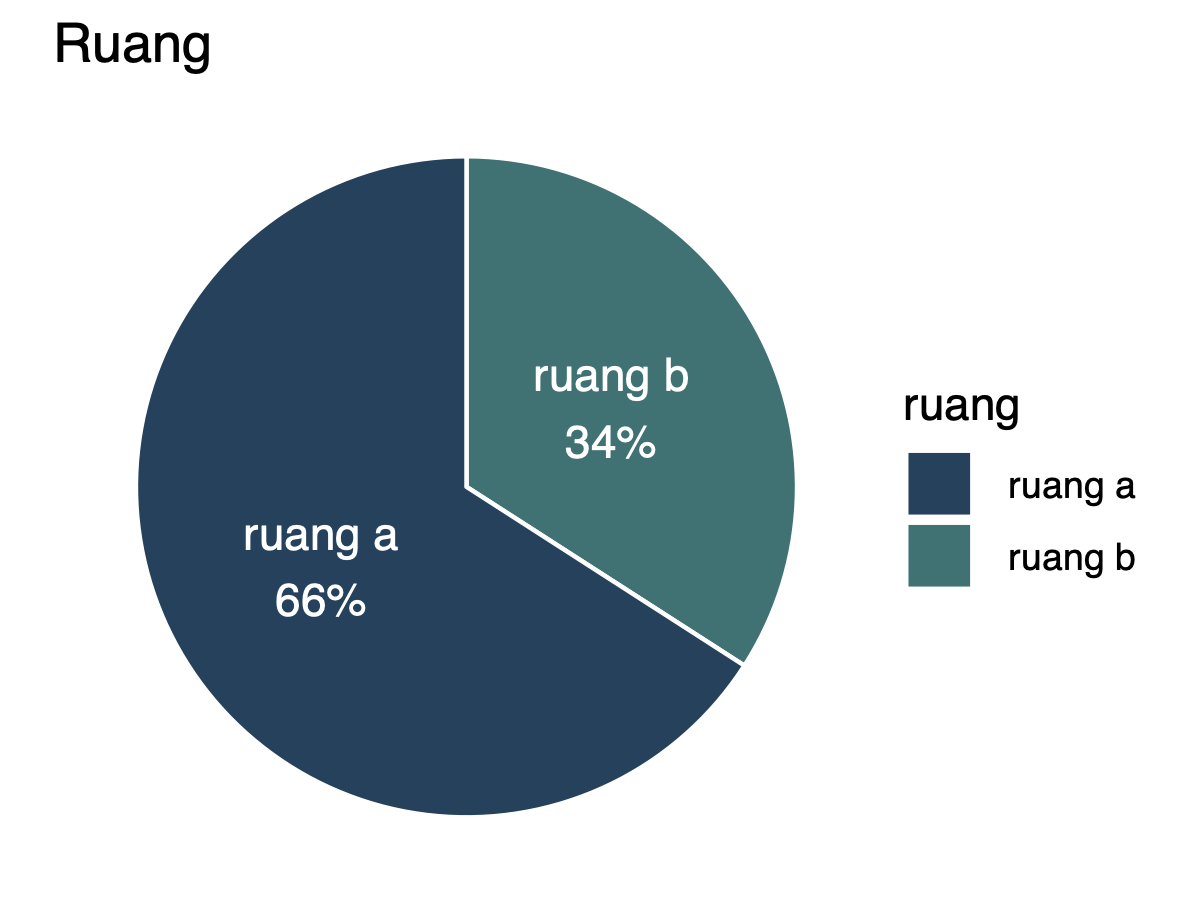
\includegraphics[width=\textwidth,trim={.4cm .3cm .4cm .1cm},clip]{figures/pieRuang.png}
    \caption{Diagram Ruang}
    \label{fig:pcr}
\end{figure}

Selanjutnya, aspek-aspek ruang digunakan untuk menganalisis alasan yang mendasari preferensi responden.
Alasan tersebut dianalisis berdasarkan aspek-aspek ruang (Definisi dan kata kunci kategori aspek dirangkum pada tabel \ref{tab:defasp} dan tabel \ref{tab:katasp}). Dari total 85 responden itu, terdapat 150 total respon yang dibagi berdasarkan kategori aspek ruang seperti: Aksesibilitas, Keamanan, Estetika dan Fasilitas. Oleh karena itu, kata kunci dari setiap kategori jawaban responden (respon) dicocokkan dengan deskripsi dan frekuensi kemunculan di setiap kategori dihitung.

\begin{table}[htpb]
    \centering
    \caption{Definisi dan sumber kategori aspek}
    \label{tab:defasp}
    \begin{tabularx}{\textwidth}{p{2.2cm} p{.45\textwidth} l}
        \toprule
        \textbf{Kategori Aspek} & \textbf{Definisi} & \textbf{Sumber}\\
\midrule
Aksesibilitas & Kemampuan individu untuk mendekati sesuatu  & \cite{larosa2018} \\
Keamanan & Bentuk perlindungan pada diri sendiri, keluarga, dan teman & \cite{carr1992} \\
Estetika & Kebutuhan akan rasa keindahan & \cite{hradilova2013} \\
Fasilitas & Penggunaan untuk memfasilitasi dan mendukung aktivitas  & \cite{carmona2021} \\
\bottomrule
    \end{tabularx}
\end{table}

\begin{table}[ht]
    \centering
    \caption{Kategori Analisis Jawaban Responden dengan Sub-kategori Aspek seperti yang Dideskripsikan oleh Responden}
    \label{tab:katasp}
    \begin{tabular}{c l}
        \toprule
        \textbf{Kategori Aspek} & \textbf{Kata kunci}\\
\midrule
Aksesibilitas & Terbuka, Tertata, Bebas, Lapang \\
Keamanan & Aman, Tanpa rasa takut\\
Estetika & Indah, Bersih, Mewah, Menarik \\
Fasilitas & Makan, Berkumpul, Duduk, Nyaman \\
\bottomrule
    \end{tabular}
\end{table}

Hasilnya menunjukkan bahwa pertama, kata seperti ``terbuka, lapang, tertata" sering diucapkan pada kategori aspek aksesibilitas. Kedua, kata seperti ``bersih, indah, mewah, dan menarik" sering muncul pada kategori aspek estetika. Ketiga, kata seperti ``tidak takut, dan aman" menjadi buah perbincangan pada aspek keamanan. Terkahir, kata seperti ``makan, duduk dan berkumpul" sering diulangi pada aspek fasilitas. Kata-kata tersebut terpilah dalam sebuah sub kategori aspek pada tabel \ref{tab:katasp}.

Sedangkan untuk frekuensi hasilnya menunjukkan bahwa dari aspek fasilitas, orang menyukai sebuah ruang yang nyaman. Dari aspek aksesibilitas, orang menyukai sebuah ruang yang luas. Alasannya orang dapat memaksimalkan pemanfaatan ruang tersebut.

Dari total 150 respon dari 85 responden terkait alasan menyukai ruang tertentu, 54\%-58\% (46-50) respon menunjukkan alasannya menyukai ruang karena aspek estetika, aksesibilitas dan fasilitas. Sedangkan hanya ada 8\% (7) respon yang beralasan aspek keamanan dalam menyukai ruang (lihat tabel \ref{tab:mrpaF}).

\begin{table}[ht]
\centering
\caption{Frekuensi aspek} 
\label{tab:mrpaF}
\begin{tabular}{llll}
  \toprule
Aspek & Frek & Pct.Resp & Pct.Kasus \\ 
  \midrule
aksesibilitas & 47 & 31.33 & 55.29 \\ 
  keamanan & 7 & 4.67 & 8.24 \\ 
  estetika & 46 & 30.67 & 54.12 \\ 
  fasilitas & 50 & 33.33 & 58.82 \\ 
  total & 150 & 100 & 176.47 \\ 
   \hline 
 \multicolumn{4}{l}{\scriptsize{sumber: Analisis,2022 }} \\
\end{tabular}
\end{table}

Selanjutnya, respon tersebut digolongkan berdasarkan macam-macam ruang yakni ruang A dan B. Hasilnya 25\% (37) responden memilih aspek estetika sebagai alasan menyukai ruang A dibandingkan dengan 20\% (30) memilih aspek fasilitas dan 21\%(32) aspek aksesibilitas. Sementara, 13\% (20) responden memilih aspek fasilitas dalam menyukai ruang B dibandingkan dengan 10\%(15) responden memilih aspek aksesibilitas dan 6\% (9) memilih aspek estetika. Meskipun demikian, terdapat preferensi yang signifikan terhadap aspek fasilitas pada kedua ruang. Sebaliknya, aspek keamanan hanya dipilih sebagian kecil responden. Hasil ini dapat dilihat pada tabel \ref{tab:ctpaE}.

\begin{table}\setlength\tabcolsep{2pt}
	\caption{Crosstabulasi 2 ruang dan aspek}
	\label{tab:ctpaE}
    \centering
\begin{tabular}[t]{rP{4.2em}P{4.2em}P{4.2em}P{4.2em}P{5em}}
    \hline

\bfseries\diagbox[innerleftsep=10pt,innerrightsep=3pt,width=7em, height=2.2cm]{Ruang}{Aspek \\Ruang} &
 {\rotatebox[origin=c]{90}{\parbox[c]{2.2cm}{\textbf{Aksesibili-tas}}}} &{\rotatebox[origin=c]{90}{\parbox[c]{2.2cm}{\textbf{Keamanan}}}}&{\rotatebox[origin=c]{90}{\parbox[c]{2.2cm}{\textbf{Estetika}}}}&{\rotatebox[origin=c]{90}{\parbox[c]{2.2cm}{\textbf{Fasilitas}}}}&{\rotatebox[origin=c]{90}{\parbox[c]{2.2cm}{\textbf{Total}}}}\\
\toprule
Ruang A  & 32 (21\%) & 5 (3\%)   & 37 (25\%) & 30 (20\%) & 104 (69\%) \\
Ruang B  & 15 (10\%) & 2 (2\%)   & 9 (6\%) & 20 (13\%) & 46 (31\%) \\
Total  & 47 (31\%) & 7 (5\%)  & 46 (31\%) & 50 (33\%) &150 (100\%) \\
 \bottomrule
\multicolumn{6}{l}{\rule{0pt}{1em}\scriptsize Sumber: Analisis, 2022 }\\
\end{tabular}
\end{table}

Hasil pada tabel crosstabulasi \ref{tab:ctpaE} kemudian digambarkan menggunakan teknik biplot untuk memahami keragaman respon aspek dan ruang. Hasilnya menunjukkan bahwa aspek aksesibilitas memiliki kontribusi besar untuk preferensi terhadap kedua ruang (lihat gambar \ref{fig:bra}).

\begin{figure}[htpb]
    \centering
    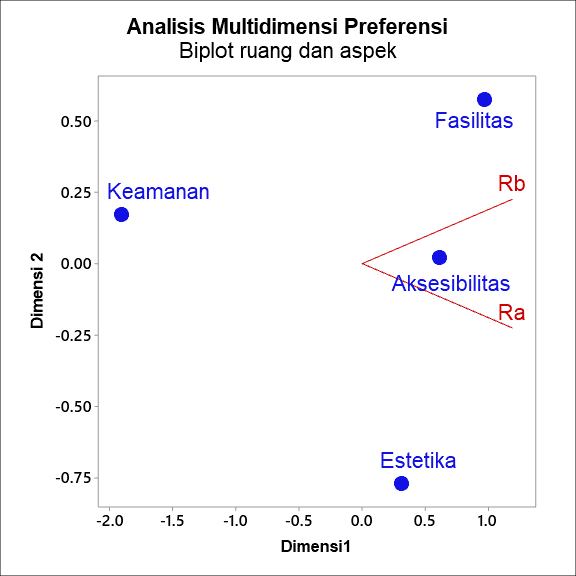
\includegraphics[width=\textwidth,trim={.4cm .3cm .4cm .1cm},clip]{figures/bra.png}
    \caption{Keragaman Preferensi terhadap Aspek dari setiap ruang}
    \caption*{Sumber: Analisis, 2022}
    \label{fig:bra}
\end{figure}


Untuk aspek aksesibilitas pada ruang A, respon dari kebanyakan responden menunjukkan bahwa kata-kata seperti `` terbuka", ``tertata", dan ``lapang" sering disebutkan. Ruang A sendiri mempunyai tempat terbuka dan tertutup. Selain itu, terdapat pula jalan pedestrian yang cukup lebar dengan penataan perabot yang tersusun cukup baik. Jalan pedestrian pada ruang ini dilindungi dengan kanopi sehingga membuat pejalan kaki terhindar dari terik matahari. Respon terhadap kondisi ruang A berkaitan dengan aspek aksesibilitas teruraikan dalam sejumlah penggalan kalimat berikut ini:

\begin{quoting}
    Ruang ini memberi kesan lapang tapi tetap memiliki estetika sehingga membuat kita menjadi nyaman ketika berada di ruang tersebut.
\end{quoting}

\begin{quoting}
    Ruang ini terlihat lebih rapi, pedestrian yang lumayan luas dan tidak banyak kendaraan yang berlalu lalang.
\end{quoting}

\begin{quoting}
    Ruangan ini memiliki jalan, sungai, dan tidak ada berjejeran motor. Jadi saya bisa berjalan disana dan melihat pemandangan tanpa ada rasa takut.
\end{quoting}

Sementara untuk aspek aksesibilitas pada ruang B, respon menunjukkan bahwa kata-kata seperti ``terbuka", ``bebas", dan ``humanis" banyak muncul pada respon. Ruang B hanya bersifat terbuka, tidak memiliki tempat yang tertutup. Meskipun demikian, itu menjadi alasan orang untuk dapat melihat jalan yang terbuka dan bisa melihat orang yang sedang beraktivitas. Pengunjung menjawab dengan macam-macam pendapat mengenai alasan memilih ruang B terkait dengan aspek aksesibilitas , beberapa diantaranya sebagai berikut:

\begin{quoting}
    Ruang terbuka dengan desain yang lebih humanis.
\end{quoting}

\begin{quoting}
    Ruang ini bisa kita melihat jalan yang terbuka dan bisa lihat orang yang sedang beraktivitas.
\end{quoting}

\begin{quoting}
    Bisa pilih-pilih makanan sesuai selera dan bisa berjalan dengan puas.
\end{quoting}

Untuk aspek estetika pada ruang A, respon banyak mengungkapkan kata-kata seperti ``indah", ``bersih", dan ``mewah". Ruang A jelas memiliki sejumlah elemen-elemen yang sangat mewah dan menarik dengan jumlah yang cukup banyak. Seperti contoh: lampu jalan, meja, dan keramik. Elemen-elemen tersebut tentunya menambah pengalaman estetika seseorang. Adapun sejumlah respon yang memilih ruang A karena estetika sebagai berikut:

\begin{quoting}
   Bisa menikmati laut lepas jauh dan menghilangkan penat...
\end{quoting}

\begin{quoting}
    Karena bersih, rapi dan memiliki pemandangan yang indah.
\end{quoting}

\begin{quoting}
    Lebih representatif dan nyaman tidak terkesan kumuh dan jorok.
\end{quoting}

Respon terkait aspek estetika juga memiliki kontribusi terhadap ruang B. Pada ruang B, orang dapat menikmati pemandangan orang berenang.Menurut \cite{mumcu2016}, orang menyukai pemandangan aktivitas orang seperti berenang. Berikut deskripsi respon responden terhadap ruang B karena estetika.

\begin{quoting}
    Ruang terbuka dengan desain yang lebih humanis.
\end{quoting}

\begin{quoting}
    Ruang ini bisa kita melihat jalan yang terbuka dan bisa lihat orang yang sedang beraktivitas.
\end{quoting}

\begin{quoting}
    Bisa pilih-pilih makanan sesuai selera dan bisa berjalan dengan puas.
\end{quoting}

Untuk aspek fasilitas, responden menunjukan respon lebih besar terhadap ruang A. Mereka mendeskripsikan dengan kata-kata seperti ``Makan", ``Berkumpul", ``Duduk". Wajar saja apabila terdapat fasilitas kedai makanan dan tempat duduk yang tertata. Adapun respon yang paling mewakili aspek fasilitas sebagai alasan memilih ruang A, sebagai berikut:

\begin{quoting}
    Kelihatan lebih bersih dan rapi jadi enak buat saya santai santai duduk.
\end{quoting}

\begin{quoting}
    Ruang ini memiliki tempat rekreasi dan refreshing sekaligus memberdayakan pedagang kaki lima yang sebelumnya tidak teratur sekarang menjadi bagus indah dan menyenangkan.
\end{quoting}

\begin{quoting}
    Ruang ini dapat digunakan oleh keluarga untuk menikmati indahnya view pantai sambil menikmati sajian makanan sesuai pesanan.
\end{quoting}

Meskipun aspek fasilitas lebih besar pada ruang A, ruang B juga menunjukkan adanya kontribusi. Kata-kata yang sering muncul pada deskripsi respon ini adalah ``Berkumpul", ``Makan", dan ``Melihat". Adapun sejumlah potongan deskripsi respon yang memilih ruang B karena aspek fasilitasnya:

\begin{quoting}
    Tempatnya bagus untuk kumpul-kumpul dengan keluarga atau teman dll, pemandangan yang bagus.
\end{quoting}

\begin{quoting}
   Karena ruangan B adalah ruangan yang cocok untuk berlibur bersama keluarga dengan makan sambil duduk disamping pantai dengan keramaian.
\end{quoting}

\begin{quoting}
    Karena bisa menikmati suasana pantai.
\end{quoting}

Selanjutnya, penelitian ini memberikan pilihan jenis-jenis elemen yang disediakan berdasarkan variabel penelitian (tabel \ref{tab:varpar}). Tujuannya untuk memahami apa saja elemen sehingga pengunjung memilih ruang tertentu. Responden meluangkan waktunya untuk memikirkan sejumlah elemen yang mereka sukai. Elemen-elemen yang mereka sukai selanjutnya dicatat.

Hasil penelitian ini menggambarkan bahwa responden sangat menyukai elemen jalan yang lebar. Sama dengan temuan-temuan sebelumnya bahwa orang mempertimbangkan aksesibilitas pada suatu ruang publik.

Dari hasil elemen-elemen yang disukai responden, terdapat 267 total respon. Selanjutnya respon tersebut digolongkan berdasarkan macam-macam ruang yang terdiri dari ruang A dan B. Hanya respon yang memiliki jumlah disukai yang relatif cukup besar akan ditampilkan pada tabel.

Pada ruang A, responden lebih menyukai lebar jalan dengan lebar tiga meter sebanyak 13\% (35) responden dibandingkan dengan responden yang menyukai beberapa pohon, permukaan aspal, permukaan keramik, pencahayaan tinggi dan elemen yang menghadap laut sebanyak 4\% (10) - 11\% (29) responden. Sementara yang menyukai elemen lainnya hanya sebesar kurang dari 3\% (8). Pada ruang B, responden lebih menyukai ruang dengan pencahayaan yang cukup sebesar 4\%(11) responden dibandingkan dengan responden yang menyukai pohon yang cukup rindang sebanyak 1\%(4). Sementara yang menyukai elemen lainnya berkisar dibawah 1\% (3), lihat tabel \ref{tab:ctpeSE}.

\begin{table}\setlength\tabcolsep{2pt}
	\caption{Crosstabulasi 2 ruang dan elemen}
	\label{tab:ctpeSE}
    \centering
    \setlength\extrarowheight{3pt}
    \begin{tabular}[ht]{P{3.4em}rP{5em}P{5em}P{5.2em} }
\hline
&\bfseries\diagbox[innerleftsep=8pt,innerrightsep=3pt,width=10em, height=2.5cm]{Elemen \\ruang}{Kelompok}


&{\bfseries\parbox[c][2.5cm]{\textwidth}{Ruang a}} &\textbf{Ruang b} & \textbf{Total}\\

\toprule

\multirow{2}{*}{\parbox{3.4em}{\textit{Jumlah pohon}}}& Sedikit pohon  & 6 (2\%)  & 3 (1\%)    &9(3\%) \\
&Beberapa pohon  &10 (4\%)  & 1     &11 (4\%) \\

\multirow{2}{*}{\parbox{3.4em}{\textit{Bentuk pohon}}}&Cukup rindang  &2 (1\%)  &4 (1\%)   &6(2\%) \\
&Sangat rindang  &28 (10\%)  & 6 (2\%)    &34(13\%) \\

\multirow{2}{*}{\parbox{3.4em}{\textit{Lebar jalan}}}&1-3m  &3 (1\%)  & 6 (2\%)   &9(3\%) \\
&> 3m  &35 (13\%)  & 7 (3\%)    &42(16\%)\\

\multirow{3}{*}{\parbox{3.4em}{\textit{Permukaan jalan}}}&Paving  &7 (3\%)  & 4 (1\%)    &11(4\%) \\
&Aspal  &12(4\%)  & 1    &13(5\%) \\
&Keramik  &12(4\%)  & 1    &13(5\%) \\

\multirow{2}{*}{\parbox{3.4em}{\textit{Jenis kursi}}}&kursi bergerak  &6(2\%)  & 0    &6(2\%)\\
&kursi dinding  &3(1\%)  & 2(1\%)    &5(2\%) \\


\multirow{2}{*}{\parbox{3.4em}{\textit{Tingkat cahaya}}}&pencahayaan cukup   &5 (2\%)  &11(4\%)     &16(6\%) \\
&pencahayaan tinggi   &31 (12\%)  & 6 (2\%)    &37(14\%)\\

\multirow{2}{*}{\parbox{3.4em}{\textit{Orientasi elemen}}}&membelakangi laut   &8(3\%)  & 3 (1\%)    &11(4\%)\\
&menghadap laut   &29 (11\%)  & 15 (6\%)    &44(16\%) \\


&Total  & 197 (74\%)  & 70 (26\%) & 267 (100\%)   \\
 \bottomrule
\multicolumn{5}{l}{\rule{0pt}{1em}\scriptsize Sumber: Analisis, 2022 }\\
\end{tabular}
\end{table}


Pada tahap selanjutnya, elemen yang ada pada tabel \ref{tab:ctpeSE} dikelompokkan menjadi 7 jenis elemen: Jumlah pohon, Bentuk pohon, Lebar jalan, Permukaan jalan, Jenis kursi, Tingkat cahaya, dan Orientasi elemen (lihat tabel \ref{tab:ctpeE}). Hasil respon elemen yang paling disukai ini selanjutnya digambarkan melalui teknik biplot untuk menerangkan keragaman preferensi terhadap elemen (lihat gambar \ref{fig:bre}).

Hasil menunjukkan terdapat perbedaan keragaman preferensi pada kedua ruang. Kontribusi terhadap ruang A lebih dominan ditunjukkan oleh jenis elemen bentuk pohon, lebar jalan, dan permukaan jalan. Sedangkan kontribusi terhadap ruang B lebih ditunjukkan oleh jenis elemen seperti tingkat cahaya dan orientasi elemen. Ruang A memiliki 4 meter lebar jalan yang mengizinkan pengunjung untuk mengakses ruang dengan mudah. Selain lebar jalan, permukaan jalan ruang ini diselimuti dengan susunan keramik yang apik. Ruang B tidak memiliki lebar jalan memadai alih-alih menggunakan bahu jalan sebagai pedestrian. Meskipun demikian, bahu jalan juga digunakan sebagai tempat parkir kendaraan. Lebih lanjut, ruang ini memiliki pemandangan teluk, orang berenang dan memancing. Kebanyakan dari mereka hanya menikmati pemandangan tersebut daripada berenang. Ruang ini menunjukkan korelasi yang cukup tinggi terlihat pada gambar \ref{fig:bre}.

\begin{figure}[htpb]
    \centering
    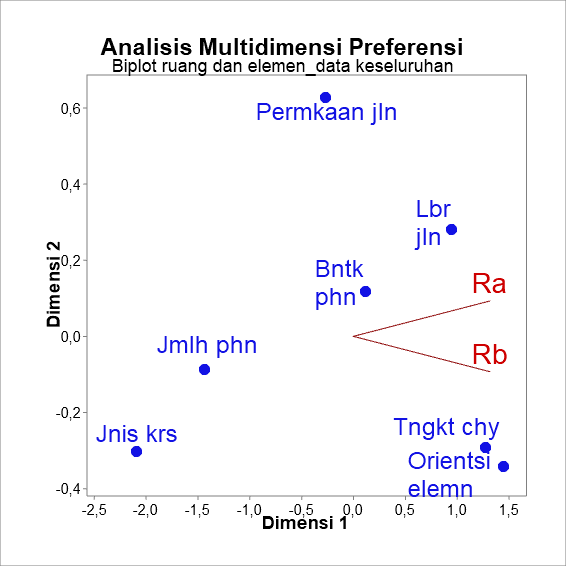
\includegraphics[width=\textwidth,trim={.5cm .3cm .5cm .1cm},clip]{figures/bre.png}
    \caption{Keragaman Preferensi terhadap elemen dari setiap ruang}
    \caption*{Sumber: Analisis, 2022}
    \label{fig:bre}
\end{figure}



\begin{table}\setlength\tabcolsep{2pt}
	\caption{Cross tabulasi ruang*kelompok elemen}
	\label{tab:ctpeE}
    \centering
\begin{tabular}[ht]{rP{5em}P{5em}P{5.5em} }
\hline
\bfseries\diagbox[innerleftsep=8pt,innerrightsep=3pt,width=10em, height=2.5cm]{Elemen \\ruang}{Kelompok}&{\bfseries\parbox[c][2.5cm]{\textwidth}{Ruang a}} &\textbf{Ruang b} & \textbf{Total}\\


\toprule

Jumlah pohon  & 16 (6\%)  & 4 (1\%) & 20 (7\%)    \\
Bentuk pohon  & 30 (11\%)  & 10 (4\%) & 40 (15\%)   \\
Lebar jalan  & 38 (14\%)  & 13 (5\%) &51 (19\%)   \\
Permukaan jalan  & 31 (12\%)  & 6 (2\%) & 37 (14\%)   \\
Jenis kursi  & 9 (3\%)  & 2 (1\%)  & 11 (4\%)  \\
Tingkat cahaya  & 36 (13\%)  & 17 (6\%) & 53 (20\%)   \\
Orientasi elemen  & 37 (14\%)  & 18 (7\%) & 55 (21\%)   \\

Total  & 197 (74\%)  & 70 (26\%) & 267 (100\%)   \\

\bottomrule

\multicolumn{3}{l}{\rule{0pt}{1em}\scriptsize Sumber: Analisis, 2022 }\\
\end{tabular}
\end{table}

\section{Kesimpulan}
Dari hasil analisis yang telah dilakukan disimpulkan bahwa pengunjung menyukai ruang A. Ruang ini terkenal dengan elemen binaan seperti lampu jalan, permukaan keramik, dan bangunan yang terpelihara. Hasil ini berbeda dengan penemuan dari \cite{zhang2006}. \cite{zhang2006} menemukan bahwa preferensi paling tinggi adalah ruang yang alami daripada ruang binaan. Oleh sebab itu, perbaikan dan peningkatan elemen buatan harus dipertimbangkan sebagai isu yang penting untuk desain dan pengelolaan ruang di tepi laut perkotaan. Orang pada ruang A lebih menyukai aspek fasilitas dan elemen dari kelompok lebar jalan. Sedangkan responden pada ruang B juga lebih menyukai aspek fasilitas, namun menyukai elemen dari kelompok orientasi elemen.
%----------------------------------------------------------------------------------------
%	BIBLIOGRAPHY
%----------------------------------------------------------------------------------------

\bibliographystyle{apacite}
\bibliography{biblioold.bib}


\end{document}
